\section{Background}
\frame{\tableofcontents[currentsection, hideothersubsections]}

\begin{frame}
\frametitle{Background: MDP}
\textbf{The environment}, $E$: \\
a Markov decision process with a state space $S$, action space $A = \mathbb{R}^N$,
an initial state distribution $p(s_1)$, transition dynamics $p(s_{t+1}|s_t, a_t)$, and
reward function $r(s_t, a_t)$.
\vspace{2.5mm}

\textbf{At each discrete timestep} $t$, \\
the agent receives an observation $x_t = s_t$ (fully observable),
takes an action $a_t$ and receives a scalar reward $r_t$.
\vspace{2.5mm}

\textbf{The return from a state}: \\
$R_t= \sum_{i=t}^T  \gamma^{(i-t)} r(s_i, a_i)$ with a discounting factor $\gamma \in [0, 1]$.
\vspace{2.5mm}

\textbf{Goal}: \\
to learn a policy, $\pi: S \mapsto P(A)$, which
maximizes $J = \mathbb{E}_{r_i,s_i \sim E,a_i \sim \pi} [R_1]$.
\vspace{2.5mm}

\textbf{Action-value function}:\\
$Q^{\pi}(s_t,a_t) = \mathbb{E}_{r_{i \ge t},s_{i>t} \sim E,a_{i>t} \sim \pi} [R_t|s_t,a_t]$.
\end{frame}

\begin{frame}
\frametitle{Background: MDP with deterministic policy}
Bellman equation (the recursive relationship):
\begin{equation}
Q^{\pi} (s_t,a_t) = \mathbb{E}_{r_{t},s_{t+1} \sim E} \Big[ r(s_t,a_t) + \gamma \mathbb{E}_{a_{t+1} \sim \pi} [Q^{\phi}(s_{t+1},a_{t+1})] \Big]
\end{equation}

If the target policy is deterministic, $\mu: S \mapsto A$, then:
\begin{equation}
Q^{\mu} (s_t,a_t) = \mathbb{E}_{r_{t},s_{t+1} \sim E} \Big[ r(s_t,a_t) + \gamma Q^{\mu}(s_{t+1},\mu(s_{t+1})) \Big]
\end{equation}

Thus:
\begin{itemize}
\item the expectation depends only on the environment $E$,
\item possible to learn $Q^{\mu}$ off-policy, using transitions which
are generated from a different stochastic behavior policy $\beta$.
\end{itemize}
\end{frame}

\begin{frame}
\frametitle{Background: Fn approximator}
Consider fn approximators parameterized by $\theta^Q$, \\
which we optimize by minimizing the loss:
\begin{equation} \label{equ:qloss}
L(\theta^Q) =\mathbb{E}_{s_t \sim \rho^{\beta}, a \sim \beta, r_t \sim E} \Big[ \Big( Q^{\phi} (s_t,a_t|\theta^Q) - y_t \Big)^2 \Big]
\end{equation}
where:\\
$y_t = r(s_t,a_t) + \gamma Q^{\mu}(s_{t+1},\mu(s_{t+1}) | \theta^Q)$, and \\
$\rho^{\beta}$: the discounted state visitation distribution for a policy $\beta$.
\vspace{5mm}

Typically, ignore the fact that $y_t$ is also dependent on $\theta^Q$.\\
\end{frame}

\begin{frame}
\frametitle{Background: Actor-critic approach}
\begin{figure}
    \centering
    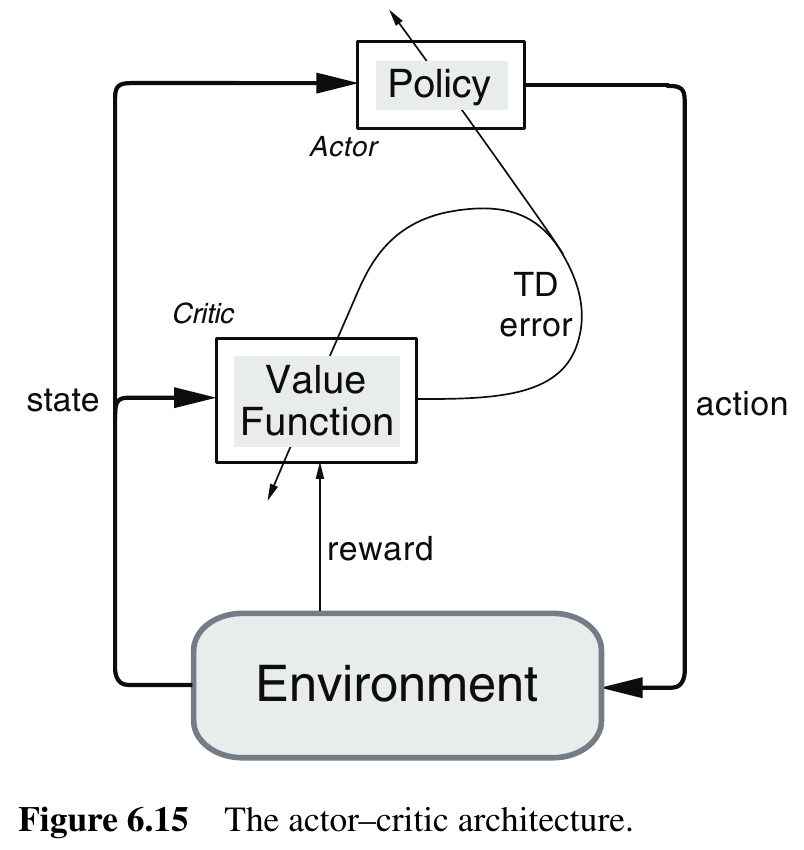
\includegraphics[scale=0.35]{actorcritic_arch}
\end{figure}
\end{frame}

% \begin{frame}
% \frametitle{Background: Actor-critic \cite{Sutton1998}}
% The Actor-Critic Algorithm is essentially a hybrid method to combine the policy gradient method and the value function method together.
% The policy function is known as the actor, while the value function is referred to as the critic.
% Essentially, the actor produces the action aa given the current state of the environment ss, while the critic produces a signal to criticizes the actions made by the actor.
% \end{frame}

% deep Q-network:
% \begin{itemize}
%   \item innovation:
%   \begin{itemize}
%     \item the network is trained off-policy with samples from a replay buffer to minimize correlations between samples;
%     the use of a replay buffer
%     \item the network is trained with a target Q network to give consistent targets during temporal difference backups.
%     a separate target network for calculating $y_t$
%   \end{itemize}
%   \item able to:
%   \begin{itemize}
%     \item solves problems with high-dimensional observation spaces,
%     \item can only handle discrete and low-dimensional action spaces.
%   \end{itemize}
% \end{itemize}
